
%%*************************************************************************
%%
%% Analysis of Biosignals by Biologically Inspired Algorithms
%% V1.0
%% 2011/05/05
%% by Peter Boraros
%% See:
%% http://www.pborky.sk/contact
%% for current contact information.
%%
%% Desription goes here.
%%
%%
%%*************************************************************************
%% Legal Notice:
%%
%% This code is offered as-is without any warranty either expressed or
%% implied; without even the implied warranty of MERCHANTABILITY or
%% FITNESS FOR A PARTICULAR PURPOSE! 
%% User assumes all risk.
%%
%% This work by Peter Boraros is licensed under a 
%% Creative Commons Attribution-NonCommercial-ShareAlike 3.0 Unported License.
%% http://creativecommons.org/licenses/by-nc-sa/3.0/


\documentclass[a4paper,jurnal]{IEEEtran}

\usepackage{cite}
% \usepackage[nocompress]{cite}
\usepackage{ifpdf}

\ifpdf
\usepackage[pdftex]{graphicx}
\graphicspath{{./img/}}
\DeclareGraphicsExtensions{.pdf}
\else
\usepackage[dvips]{graphicx}
\graphicspath{{./img/}}
\DeclareGraphicsExtensions{.eps}
\fi

\usepackage[cmex10]{amsmath}
\usepackage{amsfonts}
\usepackage{amssymb}
\interdisplaylinepenalty=2500

\usepackage{algorithmic}

\usepackage{array}

\usepackage{mdwmath}
\usepackage{mdwtab}

\usepackage{eqparbox}

% \usepackage[tight,normalsize,sf,SF]{subfigure}
\usepackage[tight,footnotesize]{subfigure}

% \usepackage[caption=false,font=normalsize,labelfont=sf,textfont=sf]{subfig}
% \usepackage[caption=false,font=footnotesize]{subfig}

\usepackage[utf8x]{inputenc}
\usepackage{url}
\usepackage{fixltx2e}
\usepackage{stfloats}
\usepackage{ucs}
\usepackage{multirow}
% correct bad hyphenation here
\hyphenation{op-tical net-works semi-conduc-tor}

% IEEEtran contains the IEEEeqnarray family of commands that can be used to
% generate multiline equations as well as matrices, tables, etc., of high
% quality.

% stfloats.sty was written by Sigitas Tolusis. This package gives LaTeX2e
% the ability to do double column floats at the bottom of the page as well
% as the top. (e.g., "\begin{figure*}[!b]" is not normally possible in
% LaTeX2e). It also provides a command:
%\fnbelowfloat
% to enable the placement of footnotes below bottom floats (the standard
% LaTeX2e kernel puts them above bottom floats). This is an invasive package
% which rewrites many portions of the LaTeX2e float routines. It may not work
% with other packages that modify the LaTeX2e float routines. The latest
% version and documentation can be obtained at:
% http://www.ctan.org/tex-archive/macros/latex/contrib/sttools/
% Documentation is contained in the stfloats.sty comments as well as in the
% presfull.pdf file. Do not use the stfloats baselinefloat ability as IEEE
% does not allow \baselineskip to stretch. Authors submitting work to the
% IEEE should note that IEEE rarely uses double column equations and
% that authors should try to avoid such use. Do not be tempted to use the
% cuted.sty or midfloat.sty packages (also by Sigitas Tolusis) as IEEE does
% not format its papers in such ways.


\begin{document}
\title{Analysis of biosignals by means of\\ biologically inspired algorithms}

\author{Peter~Boraros% <-this % stops a space
%\IEEEcompsocitemizethanks{
%	\IEEEcompsocthanksitem P. Boraros is with Department of Cybernetics, 
%		Czech Technical University, Prague, Czech Republic.\protect\\
%		E-mail: see http://www.pborky.sk/contact}
}



% The paper headers
\markboth{Peter Boraros, Czech technical university, Faculty of Electrical Engineering,
Prague, Czech Republic}%
{Shell \MakeLowercase{\textit{et al.}}: Bare Demo of IEEEtran.cls for Computer Society Journals}

\IEEEcompsoctitleabstractindextext{%
\begin{abstract}
The aim of this document is to show the usage of biologically inspired algorithms
in analysis of facial electromyography and electroencephalography.
Concretelly, it depicts the process of obtaining data, preprocessing using fast fourier
transform and classifing by means of self-organizing maps. 
Searching through the parameter space in order to find proper parametrisation of whole
classification process is performed by the genetic algorithm.
\end{abstract}}

\maketitle
\IEEEdisplaynotcompsoctitleabstractindextext
\IEEEpeerreviewmaketitle


\section{Introduction}
\IEEEPARstart{G}{oal} is to implement methods for analysis of
electromyography (EMG) and electroencephalography (EEG)
in order to allow estimation of the subject`s mimics, 
feelings or enable ability to classify the sleep stages and eventually control 
external equipment during a specific sleep stage.

This work depicts usage of self-organizing maps (SOM) as well as the usage of a genetic
algorithm (GA). It is, of course, possible to use other recognition or optimalization
techniques but usage of mentioned 
methods was induced by project assignment at a school course ``Biologically inspired 
algorithms''.

The self-ogranizing map is used  at this experiment as the method of feature recongnition in 
supervised mode. The genetic algorithm is used to guess the configuration of 
whole classification process. It searches through possible parameter ranges and 
based on value of fitness it chooses the best configuration. A fitness function
models a objectives of optimalization.

Next research will be oriented on a genetic programming. The genetic programming 
is the method of construction execution plan by similar way like genetic
algorithm. Both are inspired by nature and the process of evolution.

%Software used by this available at \url{https://github.com/pborky/biosiglab}.

\subsection{Training data, preprocessing}
Training data is usually a pulse-code modulated signal (PCM) \cite{pcm} with the
classification information attached during the signal gathering.
Sampling frequency,
can be reduced by averaging particular number of samples. Classification
information is reduced by electing a most frequent classes in given set.
Reduction is optional; it lowers the resolution but also lowers the 
computational complexity. Compromise ought to be found.

The signal is then choped into overlaping slices (windows). 
Mean value of each slice is subtracted. %TODO:why??
The signal has to be transformed %TODO: really??
from a time domain to a frequency domain.
This can be achieved by fourier-related tranforms, e.g. fourier or wavelet transform\cite{fourier,wavelet}.
The wavelet transform, unlike fourier transform, captures not only a notion of the 
frequency content of the input,
by examining it at different scales, but also temporal content.
Only fast fourier transform has been used in this work.
So, the transform ought to be aplied to each slice resulting in
a complex spectral components.
Phase information is usually discarded.
%TODO:describe possible other methods

Next the resulting vectors are subject to reduction by means of a
frequency filtering. Relevant frequency filters are problem dependent.
Figure \ref{filters2} shows aproximate ranges for some bioelectric signals.
\begin{figure}[h]
	\centering
	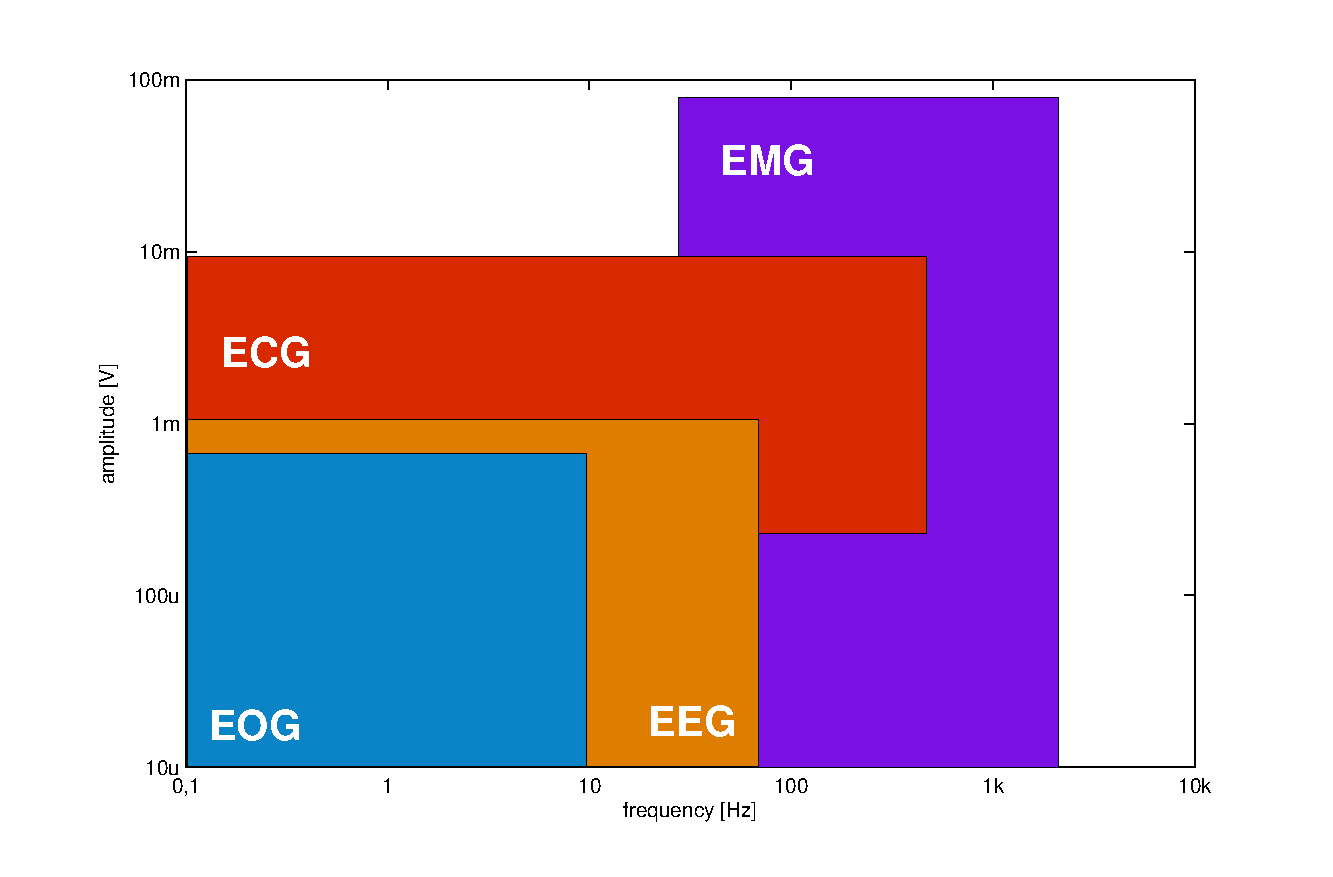
\includegraphics[width=80mm]{filters2}
	\caption{Aproximate frequency spectrums of some bioelectric signals}
	\label{filters2}
\end{figure}

Fitered spectral components are subject to normalisation/equalisation
in order to put the components
in the scale. There are several algorithms to choose. Best seems to be 
discrete histogram \cite{hist} or logistic equalization with scaling the values between 
$ \langle 0, 1 \rangle $.
Other possibilities are logaritmic or range normalisation, that normalize
values between $ \langle 0, 1 \rangle $.

The sampling frequency, window size, overlap, frequency filters and 
normalisation algorithm
are parameters ought to be sought by genetic algorithm.

\subsection{Self-organizing map}
Normalised training data (filtered spectral vectors) is then used to train 
the self-organising map.
The self-organising map is a type of artificial neural network that is
trained using unsupervised learning to produce a low-dimensional 
(typically two-dimensional), discretized representation of the input 
space of the training samples, called a map. It is method of vector 
quantisation that can be used to 
cluster analysis.
The self-organizing map consists of components called nodes or neurons. 
Associated with each node is a weight vector of the same dimension 
as the input data vectors and a position in the map space. 
The usual arrangement of nodes is a regular spacing in a hexagonal or rectangular grid. 
%More detailed information about used algorithms is available at \cite{somtoolbox}. 
The neurons with weight vectors most similar to the inputs are called 
the best matching units (BMUs).

There are two ways to interpret a SOM. 
Because in the training phase weights of the whole neighborhood are moved in the 
same direction, similar items tend to excite adjacent neurons. Therefore, 
SOM forms a semantic map where similar samples are mapped close together 
and dissimilar apart. This may be visualized by a U-Matrix 
(Euclidean distance between weight vectors of neighboring cells) of the SOM.

The other way is to think of neuronal weights as pointers to the input space. 
They form a discrete approximation of the distribution of training samples.
More neurons point to regions with high training sample concentration and 
fewer where the samples are scarce \cite{somwiki}.

This unsupervised process can be commuted to a supervised by adding a classification
information before process.
The class information is then encoded using 1-of-N encoding and appended to the 
spectral vectors. After training, the class of each map unit
is determined by taking maximum over these added components.
Finally the class information is removed \cite{somtoolbox}.

The quality of output is controled by several parameters. The most important are 
training algorithm, maps size and topografic layout and lattice.

The spatial 
layout of topological surface has to be checked. 
It should not contain irregularites; the surface ought to be ``plain''.
To quantify this criterion tolopological error is defined. It is the proportion 
of all data vectors for which first and second BMUs are not adjacent units.

Another criterion is validation/testing error. Traning set is divided into $ k $-folds
and it is trained using $ k-1 $ folds. Error is determined using the remaining fold. 
This is repeated for each fold.
Average error is the subject to minimize.

\subsection{Genetic algorithm}
A genetic algorithm (GA) is a search heuristic that mimics the 
process of natural evolution. This heuristic is routinely used to 
generate useful solutions to optimization and search problems.

In a genetic algorithm, a population of strings (called chromosomes), 
which encode candidate solutions (called individuals) to an optimization problem,
evolves toward better solutions.
Traditionally, solutions are represented in binary as strings of 0s and 1s, 
but other encodings are also possible. 
The evolution usually starts from a population of randomly generated individuals 
and happens in generations.
In each generation, the fitness of every individual in the population is evaluated,
multiple individuals are stochastically selected from the current population 
(based on their fitness), and modified (recombined and possibly randomly mutated) 
to form a new population. The new population is then used in the next 
iteration of the algorithm. 
Commonly, the algorithm terminates when either a maximum number of generations 
has been produced, or a satisfactory fitness level has been reached 
for the population. 
If the algorithm has terminated due to a maximum number of generations, 
a satisfactory solution may or may not have been reached.

A typical genetic algorithm requires:
\begin{itemize}
	\item a genetic representation of the solution domain,
	\item a fitness function to evaluate the solution domain.
\end{itemize}
A standard \textit{representation} of the solution is as an array of bits. 
Arrays of other types and structures can be used in essentially the same way. 
The main property that makes these genetic representations convenient 
is that their parts are easily aligned due to their fixed size,
which facilitates simple crossover operations. It is possible to 
represent solution by other techniques like variable array representation,
trees or graphs but the operations are more complex in that case.
The \textit{fitness function} is defined over the genetic representation and
measures the quality of the represented solution. The fitness function 
is always problem dependent.

Genetic programming (GP) is an evolutionary algorithm based methodology 
inspired by biological evolution to find computer programs that perform 
a user-defined task. 
It is a specialization of genetic algorithms (GA) where each 
individual is a computer program. 
It is a machine learning technique used to optimize a population of 
computer programs according to a fitness landscape determined by a 
program's ability to perform a given computational task \cite{gawiki}.


\section{Experiments}
\subsection{Training data} %TODO: grammar from here
Equipment used for this experiments is {Nia game controller}, made by 
{OCZ Techologies}. This device provides HID standard interface.
After it is connected, it starts to send 24-bit PCM samples, 
sampled at frequency 4kHz. The device has only one balanced channel, thus 
it is not possible to preform complex analysis of neural signals,
however for detection of EMG signal it is sufficient.

Training information is attached during the process of data gathering by human operator 
through GUI application.
The PCM data from device is saved along with class information from
user interface.

Training data contains features of facial mimics. In this experiments
following class of grimaces has beem recorded: eye-wink (left, right, both), 
relax (no grimace).
Recording time is about up to 3 minutes

\subsection{Self-organizing map}
This experiment uses implemetation of SOM based on \cite{somtoolbox}.
This implementation has wide set of options and algorithms.

Following options were analysed:
\begin{itemize}
	\item usage of \textit{batch} or \textit{sequential} training algorithm 
	\cite{somtoolbox},
	\item \textit{hexagonal} or \textit{rectangular} lattice of map,
	\item size of the map - the default number of map units is determined heuristic formula 
	$ n_{units} = 5\cdot {n_{data}}^{0.54321} $. \textit{Small} map then
	have $ 0.25\cdot n_{units} $ and \textit{big} have $ 4\cdot n_{units} $. Only
	\textit{small} and \textit{normal} is used due to to time complexity.
\end{itemize}

Figure~\ref{som_topol_proj} depicts the trained self-organizing map and traning data.
It is a PCA projection of input data vectors and BMUs.

Figure~\ref{som_umat} shows two-dimensional projection of the best matching units and
the labeling information is classification of BMUs. 
Color in U-matrix represents the distance between best matching unit. Lighter color
means larger distance and usually it depicts the division between clusters. In this case
the division is not so clearly observable. Color of labeling is following
\begin{itemize}
	\item  red - relax,
	\item green - wink (both eyes),
	\item blue - right eye wink,
	\item yellow - left eye wink.
\end{itemize}

\begin{figure}[h]
	\centering
	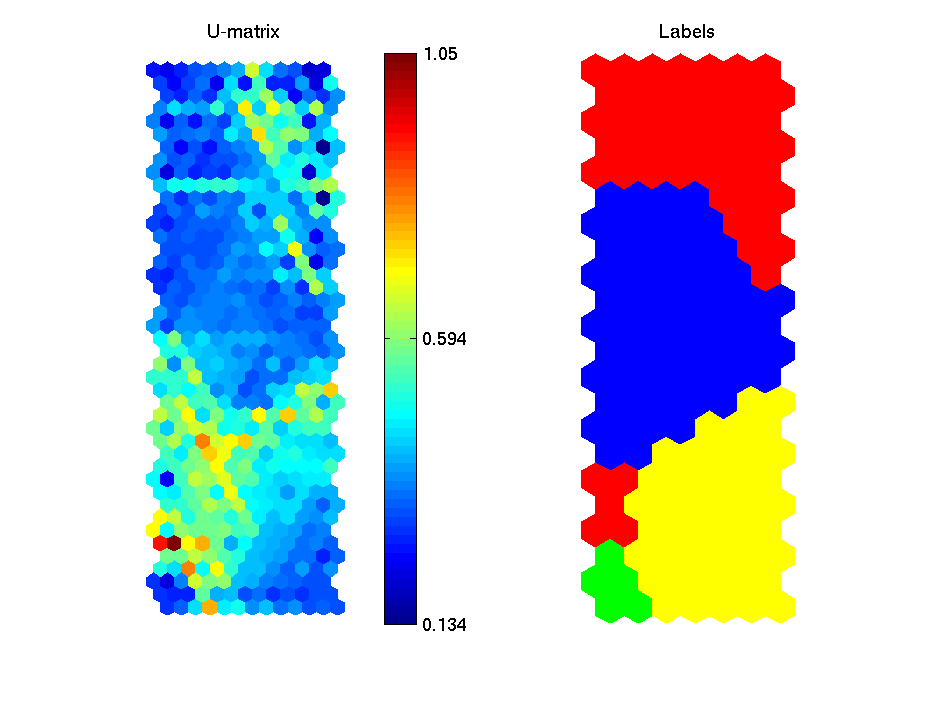
\includegraphics[width=80mm]{som_umat}
	\caption{U-matrix and classification of BMUs}
	\label{som_umat}
\end{figure}
\begin{figure}[h]
	\centering
	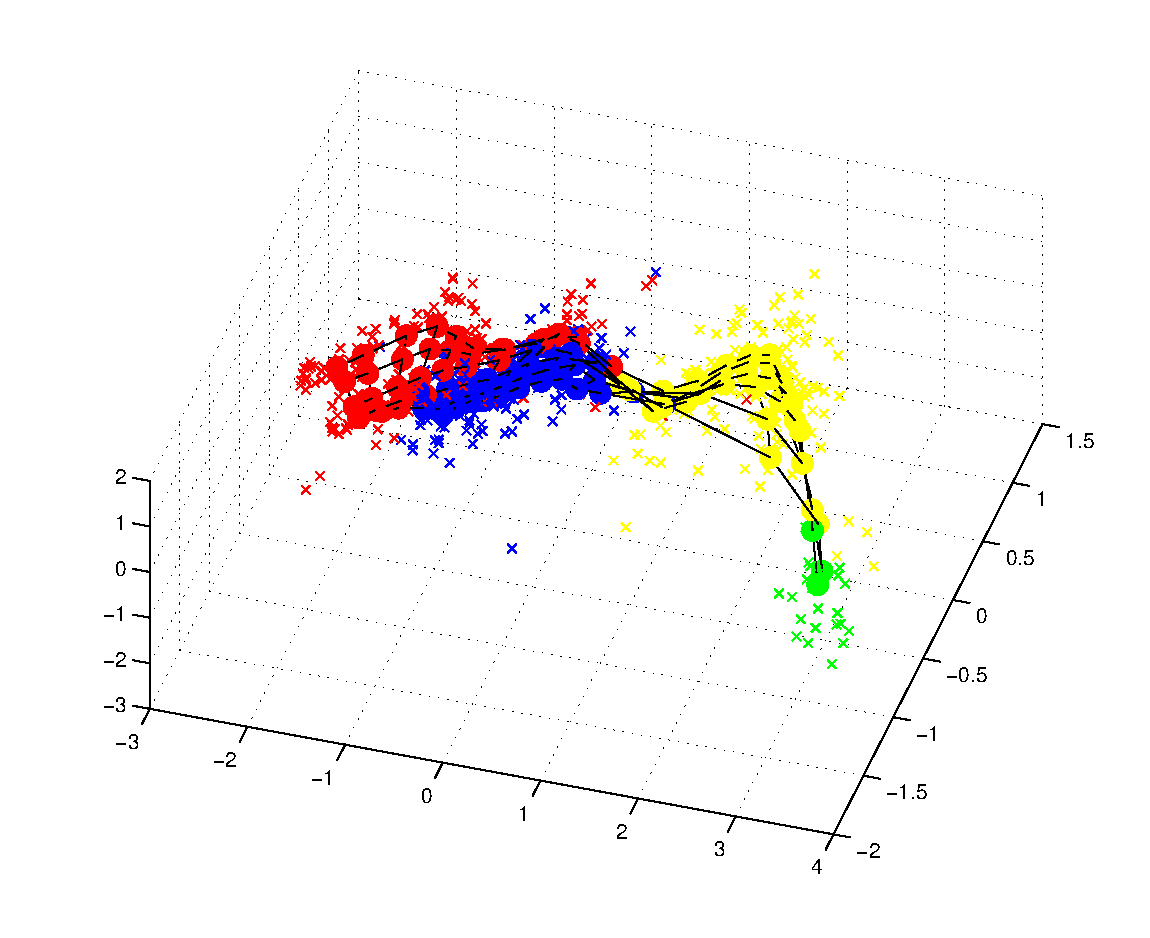
\includegraphics[width=80mm]{som_topol_proj}
	\caption{PCA Projection of topology of self-organizing map along with a data}
	\label{som_topol_proj}
\end{figure}
Figured solution has been evaluated as best-fit solution by genetic algorithm.
%TODO:tables of results, testting error

%\begin{table}[b]
%\caption{Measures of selected solutions}
%%	\begin{center}
%		\begin{tabular}[width=160mm]{|m{6mm}|m{6mm}|m{6mm}|m{6mm}|m{6mm}
%								|m{10mm}|m{10mm}|m{10mm}|m{10mm}|m{10mm}|l|l|l|l|l|l|}
%			\hline
%			\multicolumn{9}{|c|}{Parameters} & 
%			\multirow{2}{*}{val.err.} &
%			\multirow{2}{*}{test err.} &
%			\multirow{2}{*}{top.err.} &
%			\multirow{2}{*}{runtime} &
%			\multirow{2}{*}{windowsize} \\
%			\hline
%			$ f_{samp} $ & $ n_{wnd} $ & $ n_o $ & $ f_l $ & $ f_h $ &
%			norm. method & train algo & map lattice & map size \\
%			\hline
%			1333 & 800 & 8 & 20 & 200 & histD & batch & hexa & normal\\
%			\hline
%		\end{tabular}
%%	\end{center}
%\label{results}
%\end{table}

\subsection{Search space}
The whole process is controlled by several parameters.
The parameters can be determined by way of searching the search space.
Following degrees of freedom was identified:
\begin{itemize}
	\item sampling frequency $ f_{samp} $,
	\item time window before fourier transform $ n_w $,
	\item overlap of time windows $ n_o $,
	\item frequency filter after fourier tranform (interval $ \langle f_l, f_h
	\rangle $ defines portion of signal that is kept),
	\item normalisation method (\textit{histogram}, \textit{logaritmic}, 
	\textit{range}, \textit{logistic}),
	\item SOM training algorithm (\textit{batch} or \textit{sequential}),
	\item lattice of SOM (\textit{hexagonal} or \textit{rectangular}),
	\item size of SOM (depends on size of traning dataset).
\end{itemize}
\begin{table}[h]
\caption{The search space}
	\begin{center}
		\begin{tabular}{|l|| l |}
			\hline
			degree of freedom & values \\
			\hline
			\hline
			$ f_{samp} [Hz] $ & 256, 666, 1333, 4000\\
			\hline
			$ n_w $ & 80, 200, 800, 2000 \\
			\hline
			$ n_o $ & 2, 8 \\
			\hline
			$ \langle f_l[Hz], f_h[Hz] \rangle $ & $ \langle 0, 50\rangle $,  
			$ \langle 20, 250\rangle $  \\
			\hline
			normalisation & histogram, logaritmic, range, logistic \\
			\hline
			training algorithm & batch, sequential  \\
			\hline
			map lattice & hexagonal, rectangular \\
			\hline
			map size  & small, normal \\
			\hline
		\end{tabular}
	\end{center}
\label{searchspace}
\end{table}
Possible objectives are:%
\begin{itemize}
	\item validation error $ e_v $ of the trained SOM network evaluated by k-fold
	crossvalidation, $ e_v \in \langle 0, 1 \rangle $,
	\item topological error $ e_t \in \langle 0, 1 \rangle $,
	\item mean quantisation error $ e_q $,
	\item window size $ \Delta t_w $,
	\item running time $ t_r $ of whole process.
\end{itemize}
The fitness function was choosen empirically based on optimalization objectives:
\[ f = -\ln(e_v+10^{-2 }) - \ln(\Delta t_w+0.5) - (0.7\cdot e_t-0.7) - P(t_r) \]
where:\\
$ P(t) $ is sigmoid function defined as:
\[ P(t) = \frac{5}{1+10\cdot e^{6-0.15t}} \]
$ e_v $ is validation error,\\
$ e_t $ is topological error,\\
$ t_r $ is running time,\\
$ \Delta t_w $ is window time span and it can be expressed as 
\[  \Delta t_w = \frac{n_w}{f_{samp}}  \]
where:\\
$ n_w $ is number of samples within window,\\
$ f_{samp} $ is sampling frequency.
\\
\begin{figure}[h] %
	\centering
	\parbox{40mm}{
		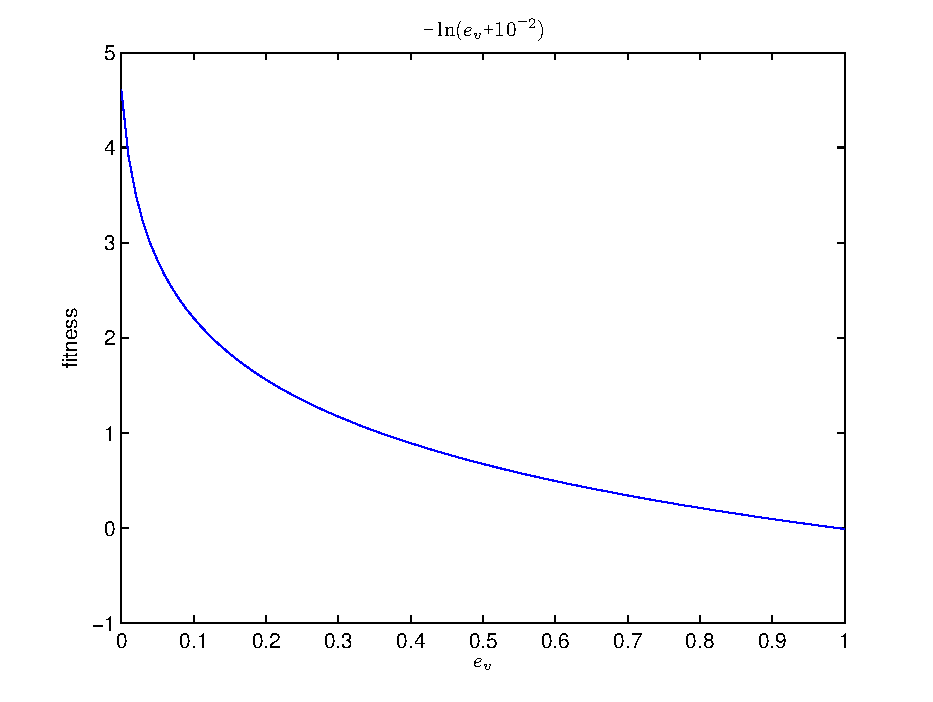
\includegraphics[width=40mm]{fit_ev}
		\caption{Validation error}
		\label{fit_ev}
	}
	\qquad
	\parbox{40mm}{
		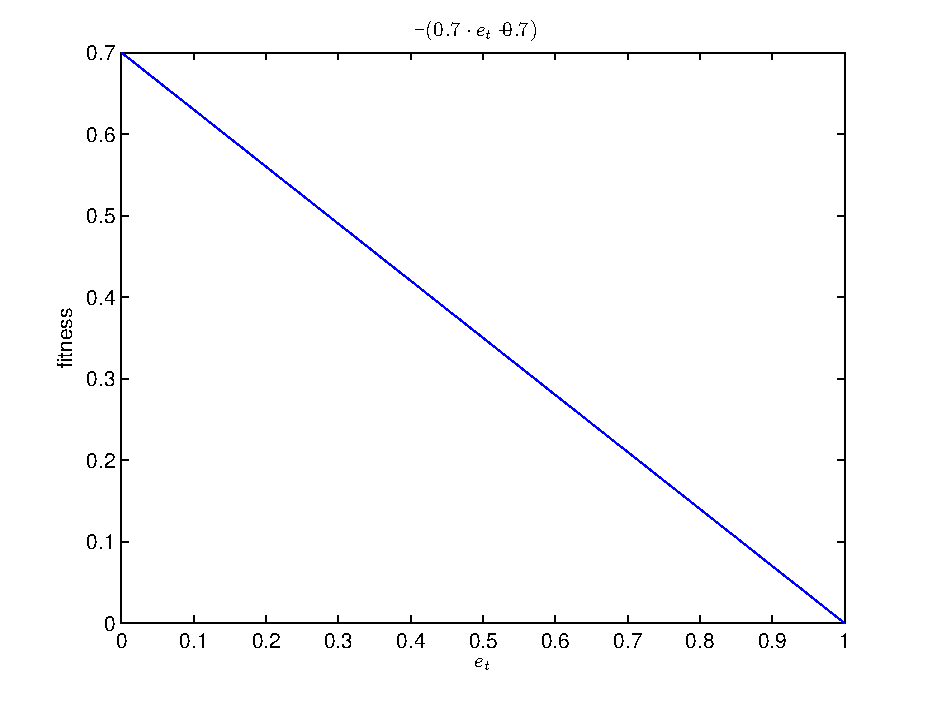
\includegraphics[width=40mm]{fit_et}
		\caption{Topological error}
		\label{fit_et}
	}
\end{figure}

Impact of particular objectives on value of fitness is following:
\begin{itemize}
	\item validation error $ -\ln(e_v+10^{-2 }) $ is the key objective and thus its impact
	ont fitness function is maximal (fig. \ref{fit_ev}),
	\item topological error $ -(0.7\cdot e_t-0.7) $ (fig. \ref{fit_et}),
	\item time window $ -\ln(\Delta t_w+0.5) $; (fig. \ref{fit_tw}),
	\item running time $ -\frac{5}{1+10\cdot e^{6-0.15t}} $ running
	time should not exceed one minute thus sigmoid function models this case (fig.
	 \ref{fit_tr}).
\end{itemize}

\begin{figure}[h] %
	\parbox{40mm}{
		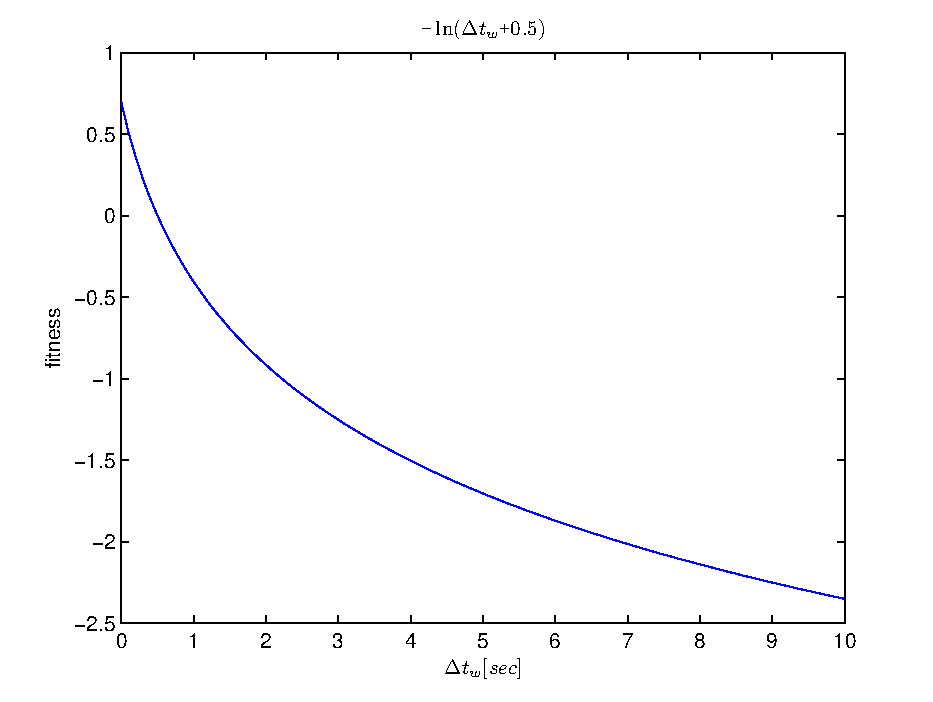
\includegraphics[width=40mm]{fit_tw}
		\caption{Time window width}
		\label{fit_tw}
	}
	\qquad
	\parbox{40mm}{
		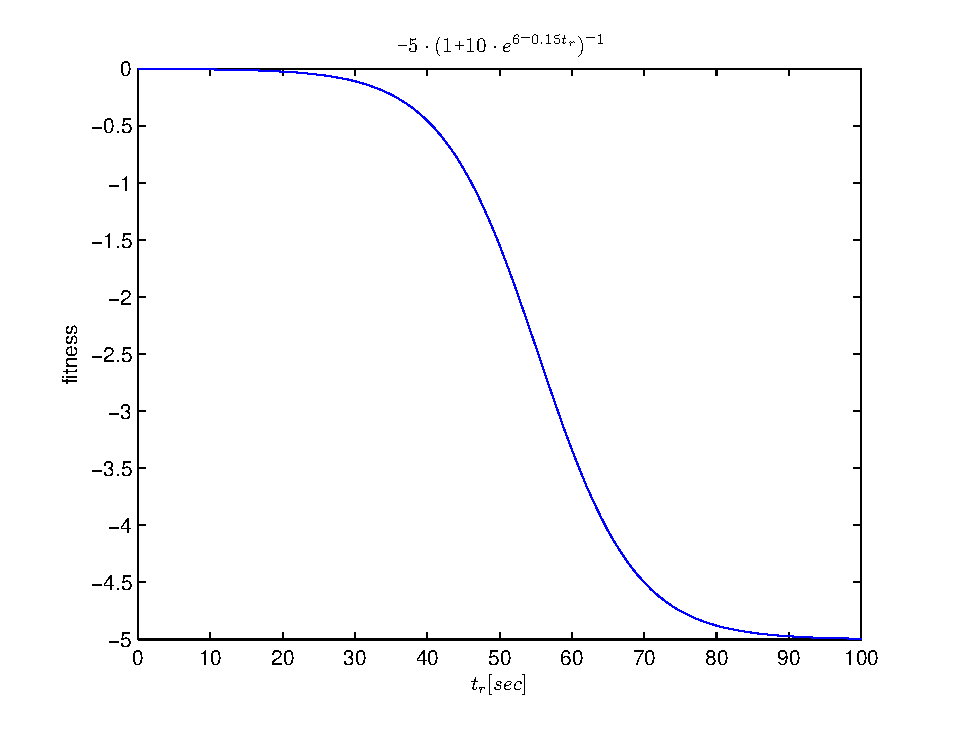
\includegraphics[width=40mm]{fit_tr}
		\caption{Running time}
		\label{fit_tr}
	}
\end{figure}

\subsection{Genetic algorithm}
Selected search space is discrete and it is listed  in table~\ref{searchspace}.%
%TODO tabular list of degrees of freedom and search space

Implementation of genetic algorithm to be introduced at this place
has following properties:

\begin{itemize}
	\item genes 
	\begin{itemize}
		\item binary strings,
		\item integer indices to the search space,
	\end{itemize}
	\item given initial population size,
	\item random uniform initialization,
	\item selection strategy:
	\begin{itemize}
		\item surviving species are selected using stochastic universal 
		sampling reducing the population size up to given initial value,
	\end{itemize}
	\item crossover:
	\begin{itemize}
		\item parents for crossover are selected using fitness proportionate
		selection of the surviving species,
		\item count of selection rounds is determined by empiric formula
		\[ N_{pr} = \lceil 0.35\cdot N_{survived} \rceil \] 		
		where $ N_{survived} $ is the number of survived species after stochastic selection.
		The value of $ N_{pr} $ limits the count of selected species.
		\item for each parent, its pair is selected by random,
		\item genes selected by random are swapped; it is uniform selection using 
		genes that are different; solution is accepted if
		produces  offsprings distinct from parents (i.e. at least one differing gene must be kept or swapped respectivelly),
	\end{itemize}
\end{itemize}
\begin{itemize}
	\item mutations:
	\begin{itemize}
		\item species for mutation are selected by 2 ways:
		\begin{itemize}
			\item using inversed-fitness proportionate
			selection from the surving species, where inverse fitness is expressed as
			$ f'=-f  $
			and count of selection rounds is
			\[ N_{mr} = \lceil n_{mr}\cdot N_{survived} \rceil \]
			where 
			$ n_{mr} $  is the rate of mutation in given population denoted as:			
			\[ n_{mr} = 0.05+\dfrac{0.25}{10\cdot e^{0.11\cdot i_{gen}-7}}\]
			where
			$ i_{gen} $ is the actual generation.\\
			The value of $ N_{mr} $ limits the count of selected species. 
			See fig. \ref{mut_r} for visualisation of relation between $ n_{mr} $ 
			and current generation.
			\item from the actual offsprings with probability of mutation for each one:
			$ P_{mo} = n_{mr} $.
		\end{itemize}
		\item each bit is flipped with fixed probability
		$ P_{mb} = 0.2 $.
	\end{itemize}
\end{itemize}
\begin{itemize}
	\item stop condition:
	\begin{itemize}
		\item fitness of best-fit species for given interval of generations has not changed.
	\end{itemize}	
\end{itemize}
\begin{figure}[h]
	\centering
	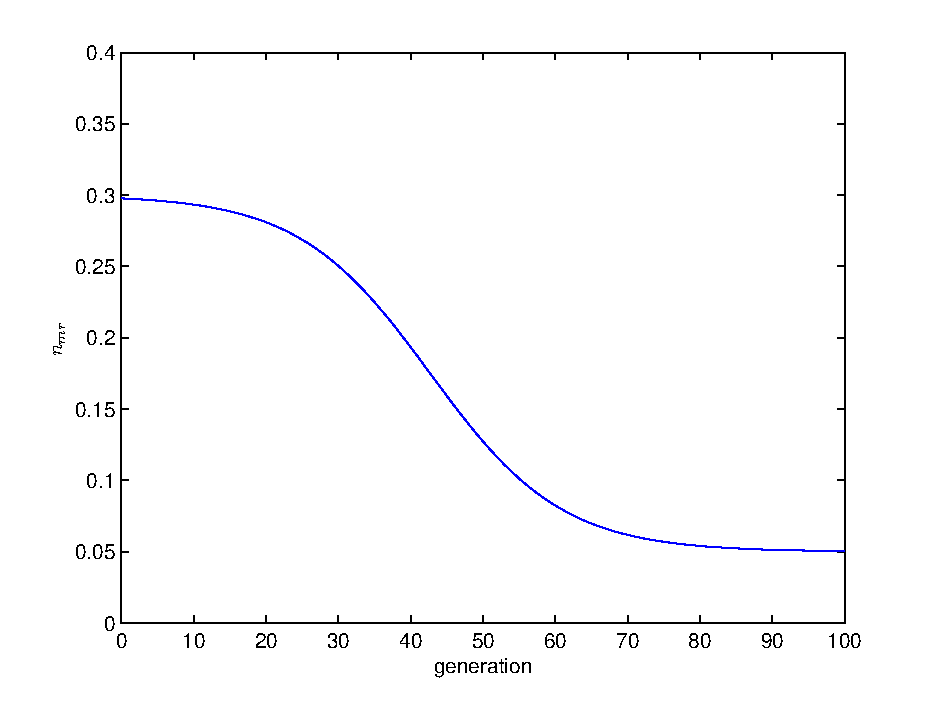
\includegraphics[width=80mm]{mut_r}
	\caption{Dependency of mutation rate on generation.}
	\label{mut_r}
\end{figure}

\subsection{Measuremenets}

\begin{figure}[h]
	\centering
	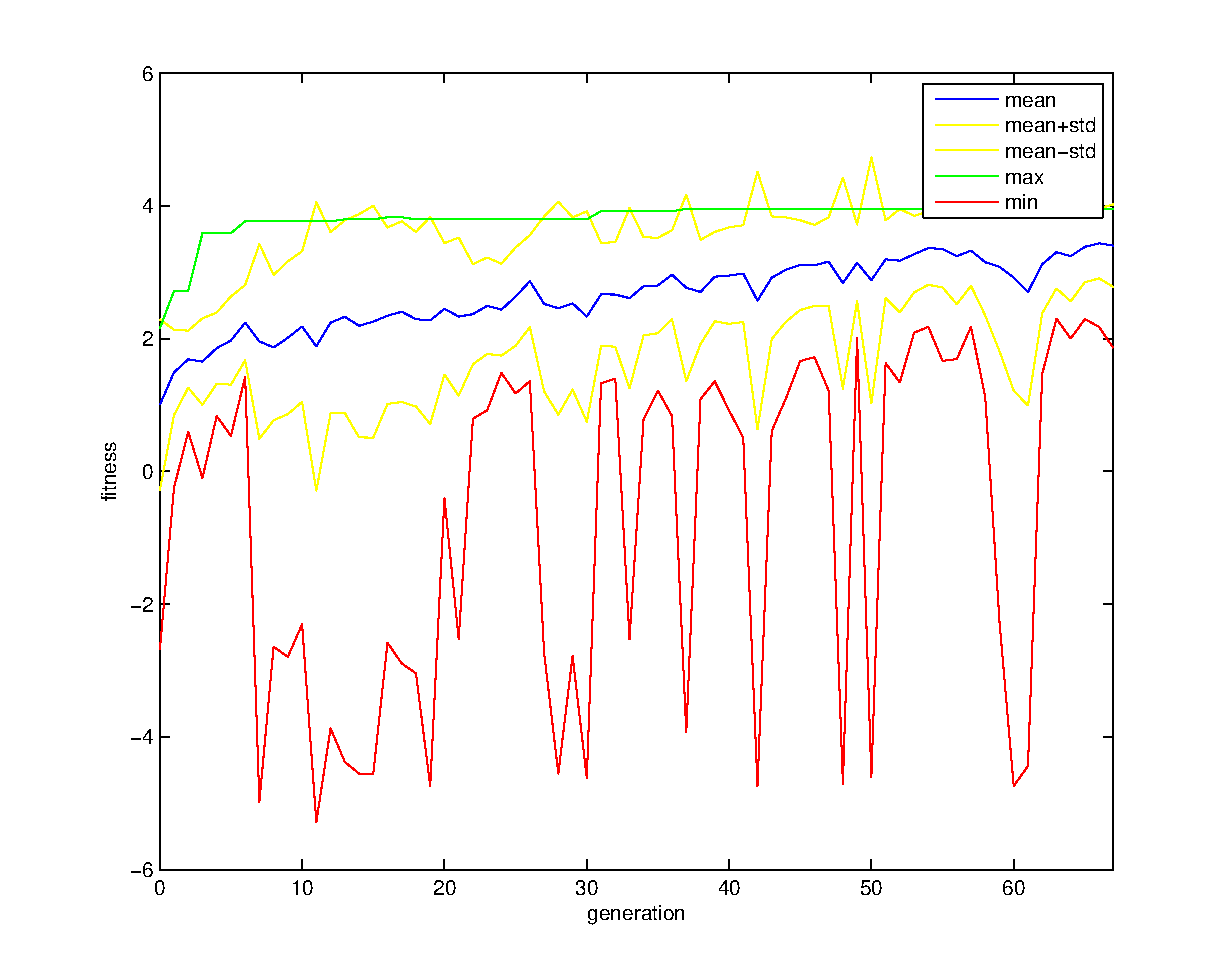
\includegraphics[width=80mm,height=55mm]{ga_conv_curve_s}
	\caption{Convergence curve of single run of GA.}
	\label{conv_curve_s}
\end{figure}
\begin{figure}[h]
	\centering
	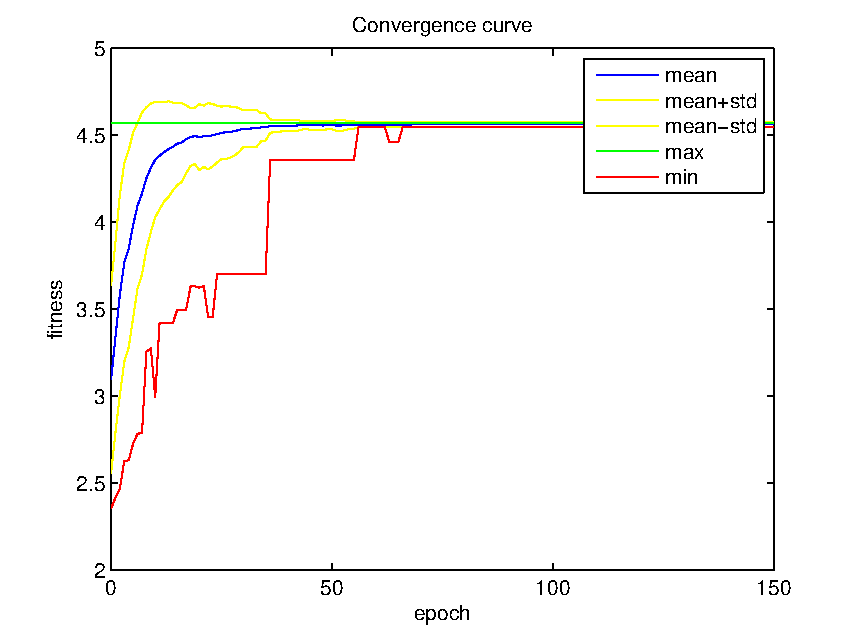
\includegraphics[width=80mm,height=55mm]{ga_conv_curve}
	\caption{Agregated convergence curve calculated on 100 runs with limit of 150 generations.}
	\label{conv_curve}
\end{figure}

% place for other SOM visualisations, and convergence curves
% convergence curve describe
% further decritption
% dependency of quality of SOM on parameters (big? table) 
% compare of best sought solution with worst

\section{Discussion}
% further decritption
% describe original tries discuss some other possibilities.


\section{Conclusion}
% what exactly measurement shows
% reference to further research : use of diferent datasets, genetic programing
% ... methods of optimisation (estimate the runnig time to avoid long running tasks)
% ... 


%TODO: consider put some big tables and figures in appendix
% if have a single appendix:
%\appendix[Proof of the Zonklar Equations]
% orsomwiki
%\appendix  % for no appendix heading
% do not use \section anymore after \appendix, only \section*
% is possibly needed

% use appendices with more than one appendix
% then use \section to start each appendix
% you must declare a \section before using any
% \subsection or using \label (\appendices by itself
% starts a section numbered zero.)
%


\appendices




% trigger a \newpage just before the given reference
% number - used to balance the columns on the last page
% adjust value as needed - may need to be readjusted if
% the document is modified later
%\IEEEtriggeratref{8}
% The "triggered" command can be changed if desired:
%\IEEEtriggercmd{\enlargethispage{-5in}}

% references section

% can use a bibliography generated by BibTeX as a .bbl file
% BibTeX documentation can be easily obtained at:
% http://www.ctan.org/tex-archive/biblio/bibtex/contrib/doc/
% The IEEEtran BibTeX style support page is at:
% http://www.michaelshell.org/tex/ieeetran/bibtex/
%\bibliographystyle{IEEEtran}
% argument is your BibTeX string definitions and bibliography database(s)
%\bibliography{IEEEabrv,../bib/paper}
%[1333]    [800]    [8]    [2x1 double]    'histD'    'batch'    'hexa'    'normal'
% <OR> manually copy in the resultant .bbl file
% set second argument of \begin to the number of references
% (used to reserve space for the reference number labels box)
\begin{thebibliography}{1}

\bibitem{somtoolbox}
Esa Alhoniemi, Johan Himberg, Juha Parhankangas, Juha Vesanto:\\
\emph{SOM Toolbox}, \hskip 1em plus
  0.5em minus 0.4em\relax http://www.cis.hut.fi/projects/somtoolbox/

\bibitem{somwiki}
  \emph{Self-organizing map}, \hskip 1em plus 0.5em minus 0.4em\relax \url{http://en.wikipedia.org/wiki/Self_organizing_maps}
  
\bibitem{gawiki}
  \emph{Genetic algorithm}, \hskip 1em plus 0.5em minus 0.4em\relax \url{http://en.wikipedia.org/wiki/Genetic_algorithms}

\bibitem{pcm}
\emph{Pulse-code modulation}, \hskip 1em plus 0.5em minus 0.4em\relax \url{http://en.wikipedia.org/wiki/PCM}

\bibitem{fourier}
\emph{Fourier transform},  \hskip 1em plus 0.5em minus 0.4em\relax \url{http://en.wikipedia.org/wiki/Fast_Fourier_transform}

\bibitem{wavelet}
\emph{Wavelet transform}, \hskip 1em plus 0.5em minus 0.4em\relax \url{http://en.wikipedia.org/wiki/Wavelet_transform}

\bibitem{hist}
\emph{Histogram equalization}, \hskip 1em plus 0.5em minus 0.4em\relax \url{http://en.wikipedia.org/wiki/Histogram_equalization}


%TODO: more references 

\end{thebibliography}

% biography section
% 
% If you have an EPS/PDF photo (graphicx package needed) extra braces are
% needed around the contents of the optional argument to biography to prevent
% the LaTeX parser from getting confused when it sees the complicated
% \includegraphics command within an optional argument. (You could create
% your own custom macro containing the \includegraphics command to make things
% simpler here.)
%\begin{biography}[{\includegraphics[width=1in,height=1.25in,clip,keepaspectratio]{mshell}}]{Michael Shell}
% or if you just want to reserve a space for a photo:



% that's all folks
\end{document}
